\begin{figure}[H]
	\centering
	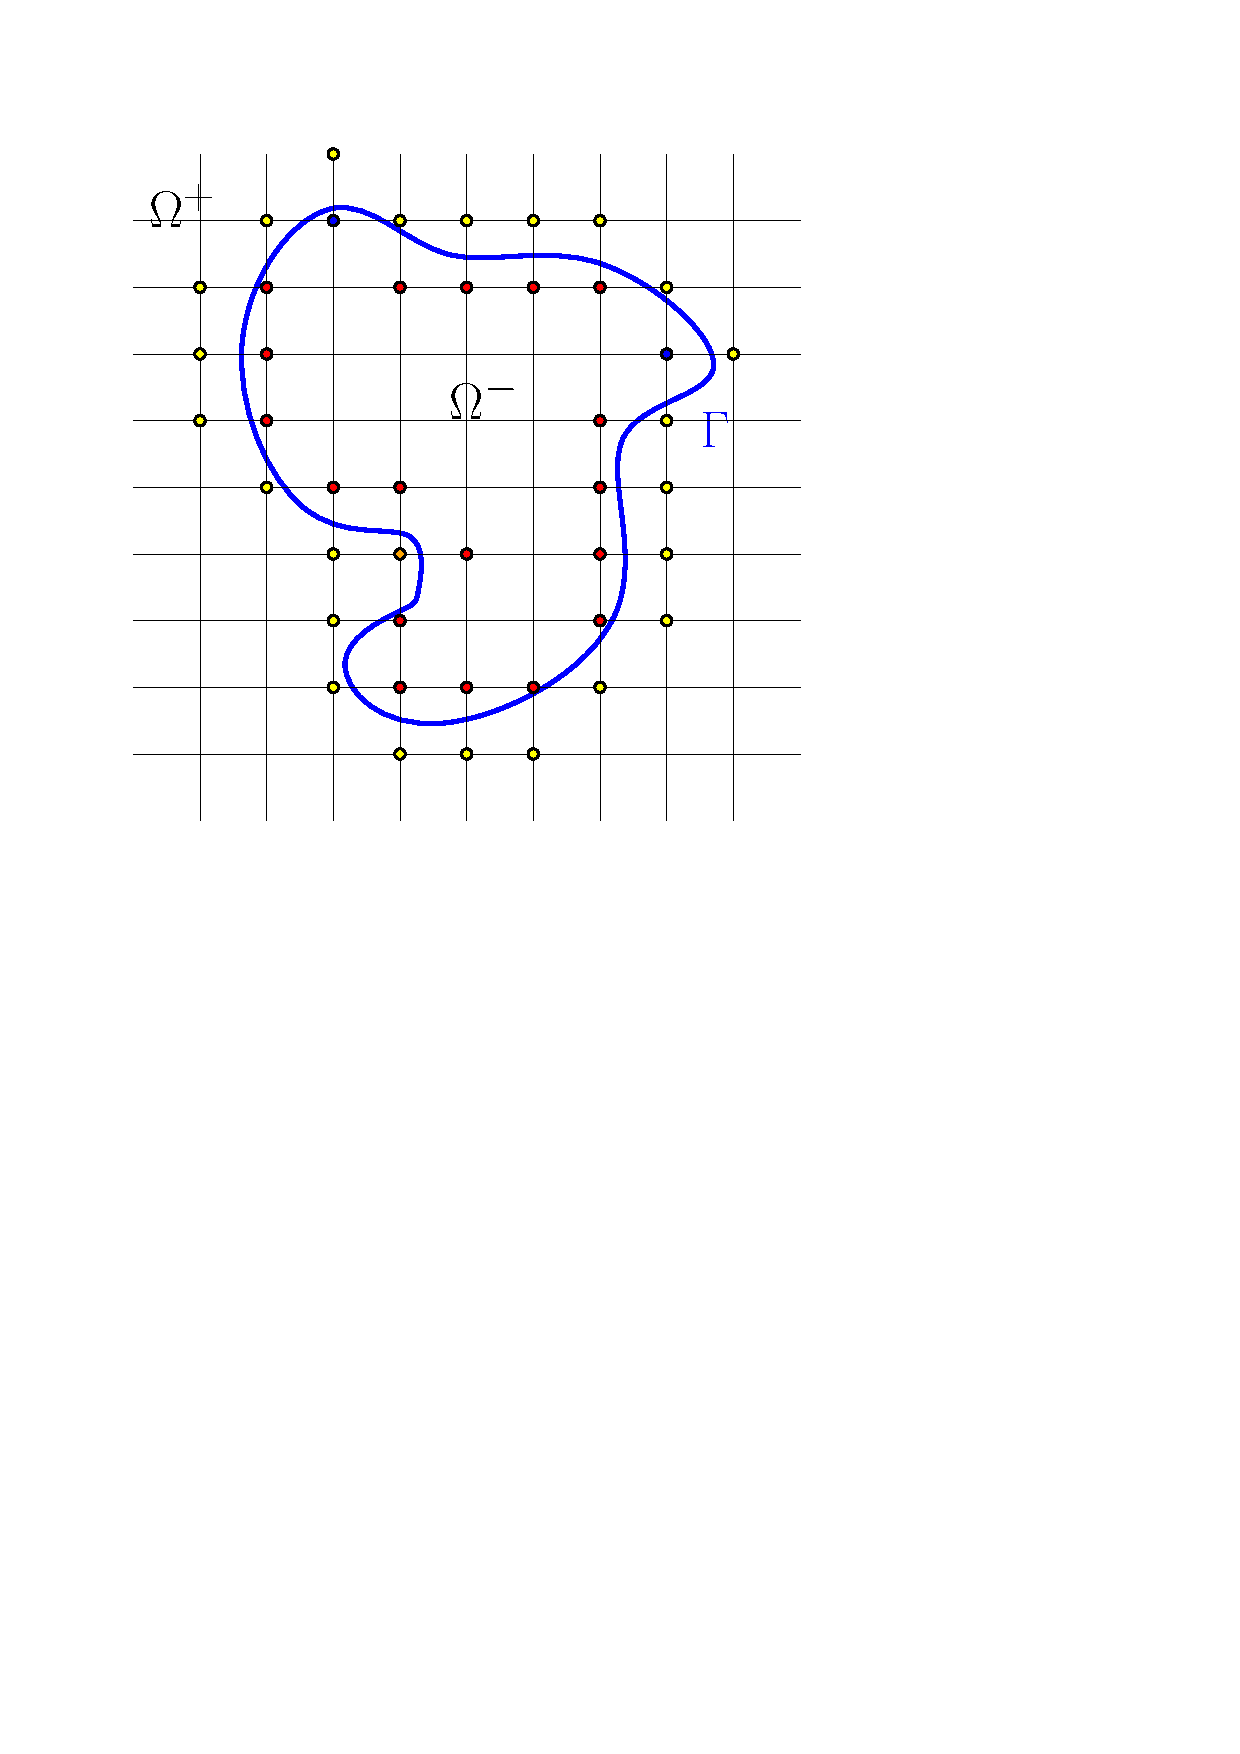
\includegraphics[scale = .7]{PBE1_grid.pdf}
	\caption{Irregular grid points marked as colored disks with blue and orange color for the corner points.}
	\label{fig_irgpoints}
\end{figure}


%on the points far away from the interface $\Gamma$ which are defined as regulars nodes.
At the points adjacent to the interface $\Gamma$, the central difference operators defined in (\ref{dif_opx})-(\ref{dif_opz}) are not used since these points are defined as irregular points where at-least one of its adjacent points is on the other side of the interface $\Gamma$. 
%On the irregular points at least one of the three point stencils for $\delta_x^2,\delta_y^2$ and $\delta_z^2$ is across the interface. 
Here the information about the function $v$ is not available for the point which is on the other side of the interface. A non-standard finite difference formula is necessary on the irregular points to discretize $\delta_x^2,\delta_y^2$ and $\delta_z^2$.  In this regard a modified version of the Ghost Fluid Method is proposed in this chapter using fictitious points (or ghost points) and the jump conditions given by (\ref{phitilde3}) and (\ref{phitilde4}).


The Ghost Fluid Method(GFM) is a sharpe interface technique introduced in  \cite{Fedkiw1999} to treat the two-face contact discontinuities in the Euler equations. It extends values across the interface into an artificial fluid (ghost fluid), inducing the jump conditions at the interface. This GFM method was later extended in \cite{Liu2000} to solve elliptic equations with variable coefficients. But in contrast to their method \cite{Liu2000}, the jump conditions are incorporated into the numerical discretization in such a way that the symmetry of the finite difference stencil is preserved. Which makes it compatible with most standard solvers. The flux jump has been decomposed in each axis direction treating the problem dimension by dimension. As a result this extended GFM becomes only first order accurate.   

%%%%%%%%%%%%%%%%%%%%%%%%%%%%%%%%%%%%%%%%%%%%%%%%%%%%%%%%%%%%%%%%%%%%%%%%%%%%%

\section{One dimension}

For a one dimensional representation of the proposed GFM schemes we try to evaluate the finite difference operator $\delta_{xx}$ at the irregular points where the interface is at $x_\Gamma$ between $x_i$ and $x_{i+1}$ as shown in Figure \ref{fig_1}.  %$x_i \leq x_\Gamma\leq x_{i+1}$.   
\begin{figure}[t!]
\begin{center}
%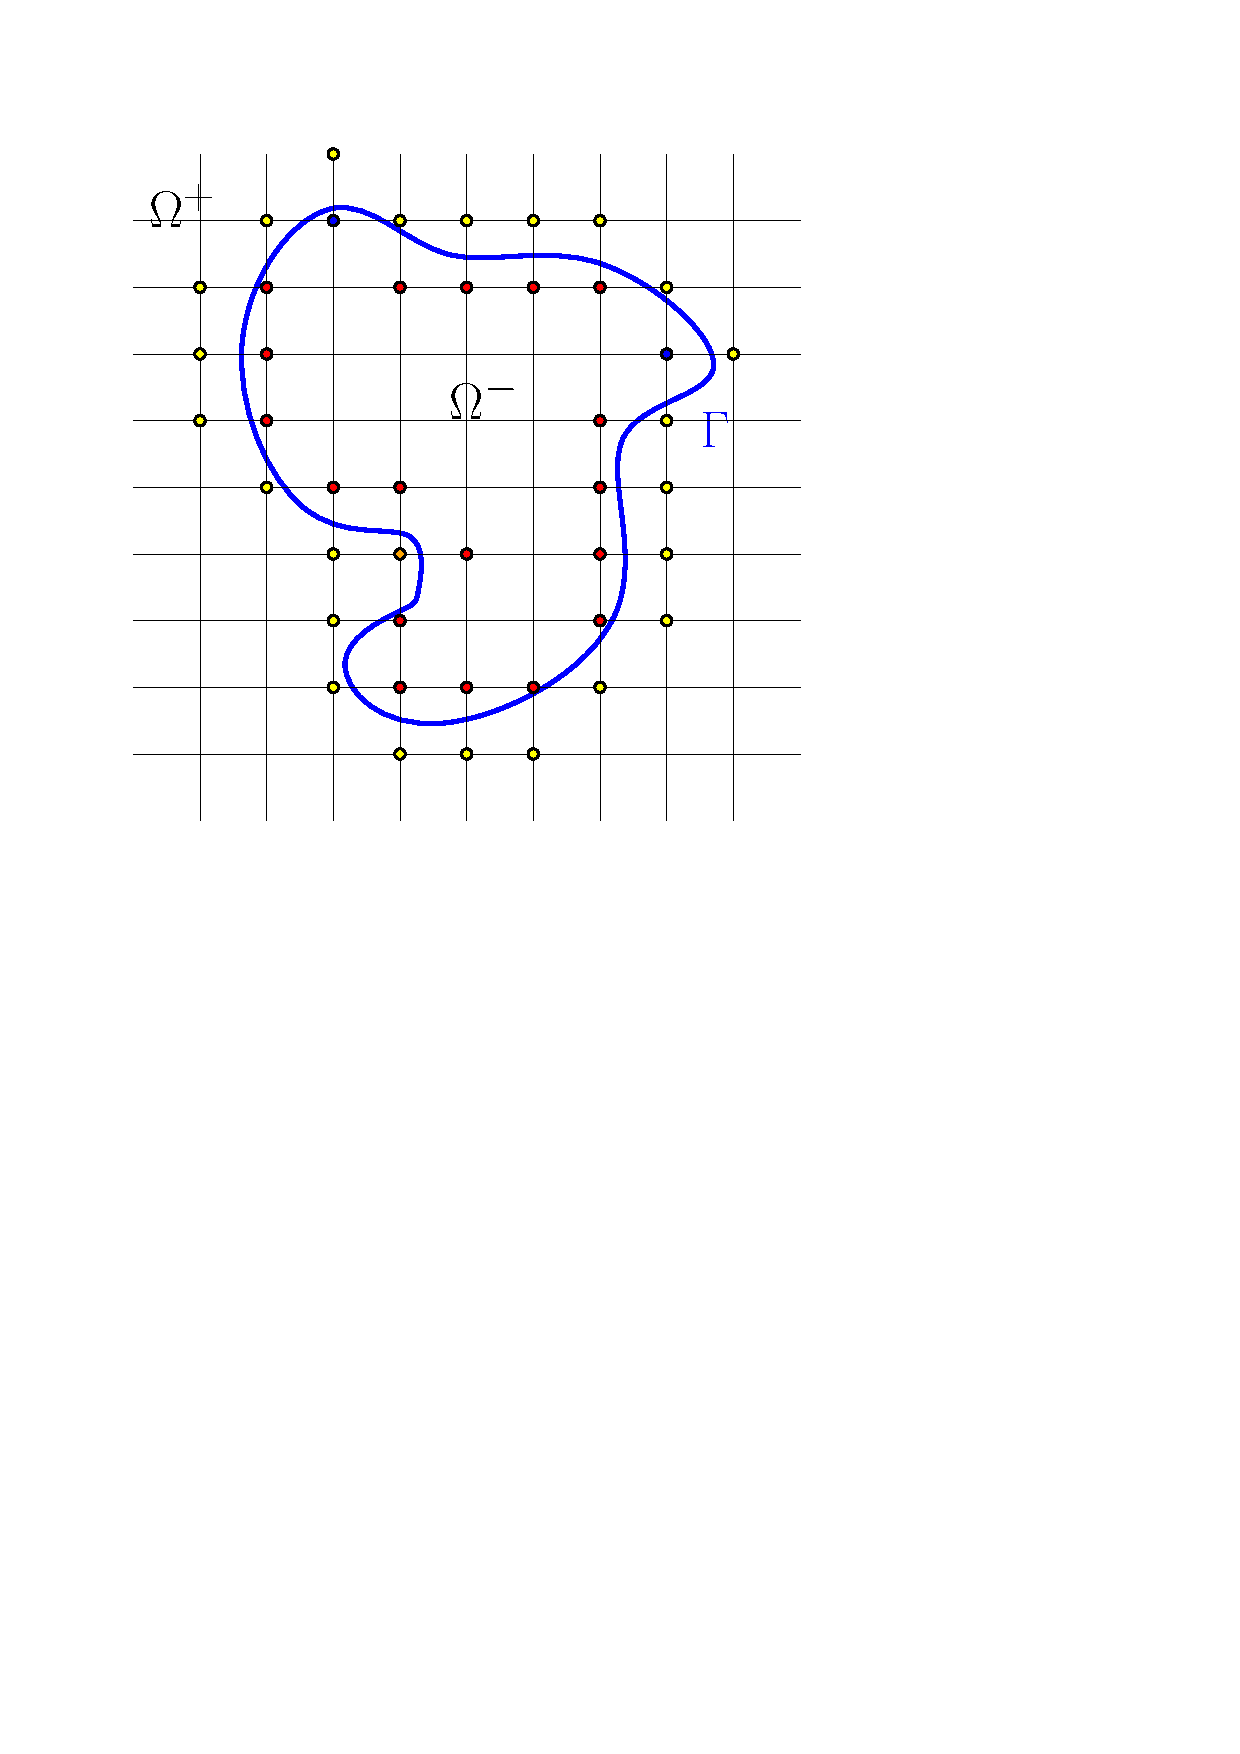
\includegraphics[scale = .5]{PBE1_grid.pdf}
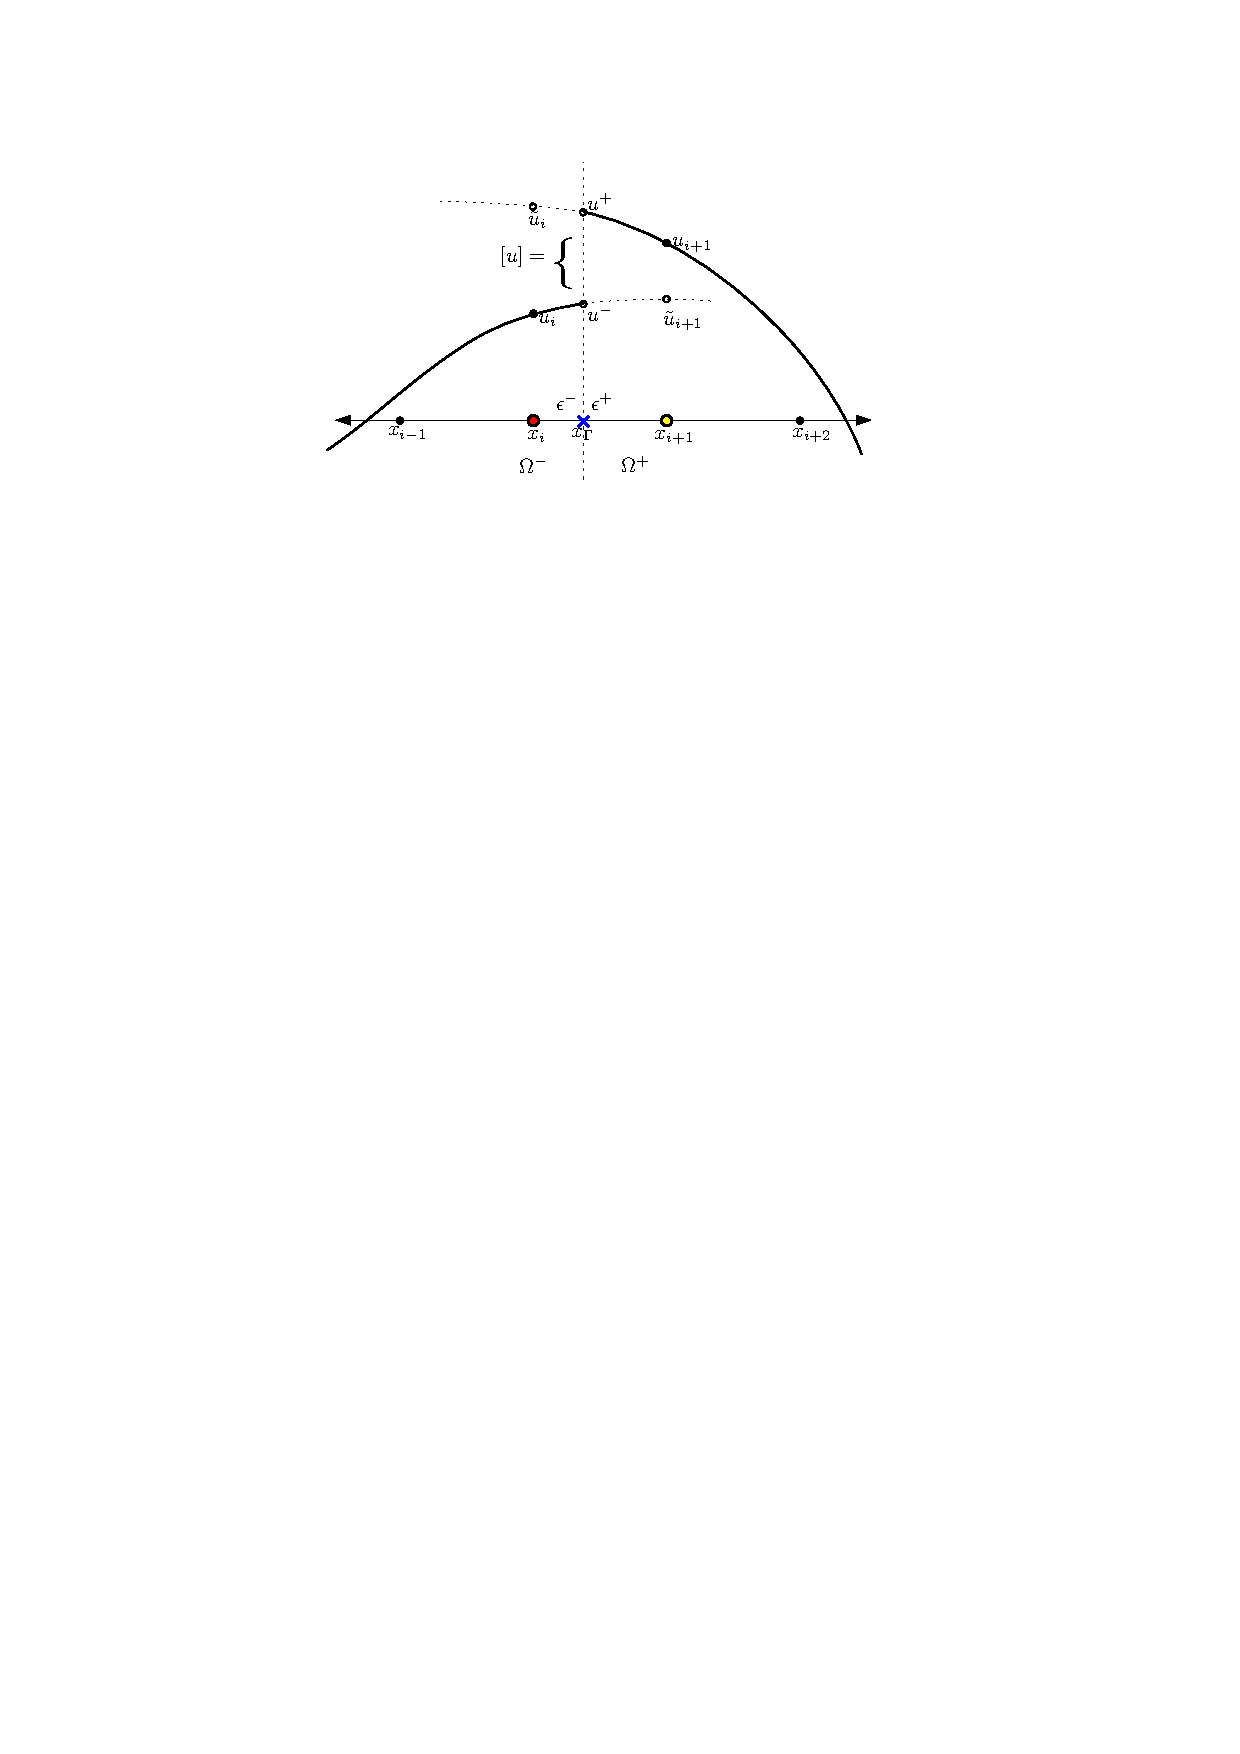
\includegraphics[scale=1.5]{1dmib1.pdf}\hspace{10mm}
\caption{1D GFM. Red and Blue colored points are the irregular points.}
\label{fig_1}
\end{center}
\end{figure}

Here $u$ satisfies the PBE as $u = u_{in} \text{ in }\Omega^-$ with $ u= u_{out}\text{ in }\Omega^+$
%$u=\begin{cases}
%u_{in} \text{ in }\Omega^-\\
%u_{out}\text{ in }\Omega^+\\
%\end{cases}$ 
and we define $u^+ = u_{out}(x_\Gamma),u^- = u_{in}(x_\Gamma),h=x_{i+1}-x_i$ and  $\lambda =\frac{x_\Gamma-x_i}{h}$ to get following equations,
\begin{eqnarray}
\begin{aligned}
x_\Gamma &= x_i + \lambda h,  \\
u^- &= u_i(1-\lambda )+ \tilde{u}_{i+1} \lambda \text{ and }u^+ = \tilde{u}_i(1-\lambda )+ u_{i+1}\lambda,\\
\left[u\right]  & = u^+-u^- \text{ and }\left[ \epsilon \frac{\partial u}{\partial x} \right] =  \epsilon^+ u^+_x-\epsilon^- u^-_x,
\end{aligned}\label{1d_GFM}
\end{eqnarray}
	
where $\tilde{u_i}$ and $\tilde{u_{i+1}}$ are the fictitious values(or ghost values) of $u$ at the irregular points extending $u_{in}$ or $u_{out}$ on the other side of the interface. In particular as shown in Figure \ref{fig_1},  we have $\tilde{u}_i \approx u_{out}(x_i)$ and $\tilde{u}_{i+1}\approx u_{in}(x_{i+1})$. Here $u_{out}$ has been extended to the point $x_i$ for $\tilde{u_i}$ and $u_{in}$ has been extended to the point $x_{i+1}$ for $\tilde{u_i}$. 

Our purpose here is to apply the non-standard finite difference operator $\delta_x^2$ at $x_i$ and $x_{i+1}$ to get: 
\begin{equation}
\delta_x^2\left(u_{i}\right)= \frac{\epsilon^-}{h^2} \left(u_{i-1}-2u_{i}+\tilde{u}_{i+1}\right)\text{ and }\delta_x^2\left(u_{i+1}\right)= \frac{\epsilon^+}{h^2} \left(\tilde{u}_{i}-2u_{i+1}+u_{i+2}\right).	\label{fnt-op}
\end{equation}
Now solving the equations in (\ref{1d_GFM})  for $\tilde{u}_i $ and $\tilde{u}_{i+1}$ we get, 
\begin{eqnarray}	\tilde{u}_i&=& \frac{\epsilon^-}{\epsilon^+\lambda+\epsilon^-(1-\lambda)}u_i +\frac{\lambda(\epsilon^+-\epsilon^-)}{\epsilon^+\lambda+\epsilon^-(1-\lambda)}u_{i+1}\nonumber\\ &+&\frac{\epsilon^-}{\epsilon^+\lambda+\epsilon^-(1-\lambda)}\left[u\right] -\frac{h \lambda}{\epsilon^+\lambda+\epsilon^-(1-\lambda)}\left[ \epsilon \frac{\partial u}{\partial x} \right],
\end{eqnarray}
and 
\begin{eqnarray}		
	\tilde{u}_{i+1}&=& \frac{(\epsilon^--\epsilon^+)(1-\lambda)}{\epsilon^+\lambda+\epsilon^-(1-\lambda)} u_i +\frac{\epsilon^+}{\epsilon^+\lambda+\epsilon^-(1-\lambda)} u_{i+1}\nonumber \\
	&-&\frac{\epsilon^+}{\epsilon^+\lambda+\epsilon^-(1-\lambda)} \left[u\right] -\frac{h(1-\lambda)}{\epsilon^+\lambda+\epsilon^-(1-\lambda)}\left[ \epsilon \frac{\partial u}{\partial x} \right].\label{u_fact}
\end{eqnarray}
Then substituting equation (\ref{u_fact}) into equation (\ref{fnt-op}) we get
\begin{equation}
		\delta_x^2\left(u_{i}\right)= \frac{1}{h^2} \left(a_1u_{i-1}+b_1 u_{i}+c_1u_{i+1}\right)+\frac{\epsilon^-}{h^2}\left(e_1.[u]+f_1.\left[ \epsilon \frac{\partial u}{\partial x} \right]\right),\label{fnt-op-1}
\end{equation}
and 
\begin{equation}		
		\delta_x^2\left(u_{i+1}\right)= \frac{1}{h^2} \left(a_2u_{i}-b_2u_{i+1}+c_2u_{i+2}\right)+\frac{\epsilon^+}{h^2}\left(e_2.[u]+f_2.\left[ \epsilon \frac{\partial u}{\partial x} \right]\right),\label{fnt-op-2}
\end{equation}
where,
\begin{eqnarray}
\begin{aligned}
d&=\epsilon^+\lambda+\epsilon^-(1-\lambda),\\
a_1&= \epsilon^-,b_1=-\epsilon^-\left(1+\frac{\epsilon^+}{d}\right), c_1=\frac{\epsilon^-\epsilon^+}{d}, e_1=\frac{\epsilon^-}{d},f_1=\frac{h\lambda}{d},\\
a_2&= \frac{\epsilon^+\epsilon^-}{d},b_2=-\epsilon^+\left(1+\frac{\epsilon^-}{d}\right), c_2=\epsilon^+, e_2=-\frac{\epsilon^+}{d},f_2=\frac{h(1-\lambda)}{d}.
\end{aligned}
\end{eqnarray}
Here, the second terms of the equations in (\ref{fnt-op-2}) are known. Only the coefficients in the 1st terms of (\ref{fnt-op-2}) contribute to the finite difference operator matrix keeping it tridiagonal to make it diagonally dominant(as $|b_1|-a_1-c_1=0\text{ and } |b_2|-a_2-c_2=0$) and symmetric (as $a_2=c_1$).  
%%%%%%%%%%%%%%%%%%%%%%%%%%%%%%%%%%%%%%%%%%%%%%%%%%%%%%%%%%%%%%%%%%%%%%%%%%%%%

  
\section{Two dimensions}
For the two dimensional PB model, we need to evaluate $\delta_{xx}$ and $\delta_{yy}$, 
where $\delta_{yy}$ can be calculated at irregular points in a manner similar to (\ref{fnt-op-2}) 
%where the similar derivation of the equations in (\ref{fnt-op-2}) can be used to calculate $\delta_{yy}$ at irregular points. 
In this case,  $\left[ \epsilon \frac{\partial u}{\partial x} \right]$ and $\left[ \epsilon \frac{\partial u}{\partial y} \right]$ are not known, while $\left[ \epsilon \frac{\partial u}{\partial n} \right]$ is given. Now to get $\left[ \epsilon \frac{\partial u}{\partial x} \right]$ and $\left[ \epsilon \frac{\partial u}{\partial y} \right]$ in terms of $\left[ \epsilon \frac{\partial u}{\partial n} \right]$ and $\left[ \epsilon \frac{\partial u}{\partial \tau} \right]$ we have the following relations,  
\begin{figure}[ht]
\begin{center}
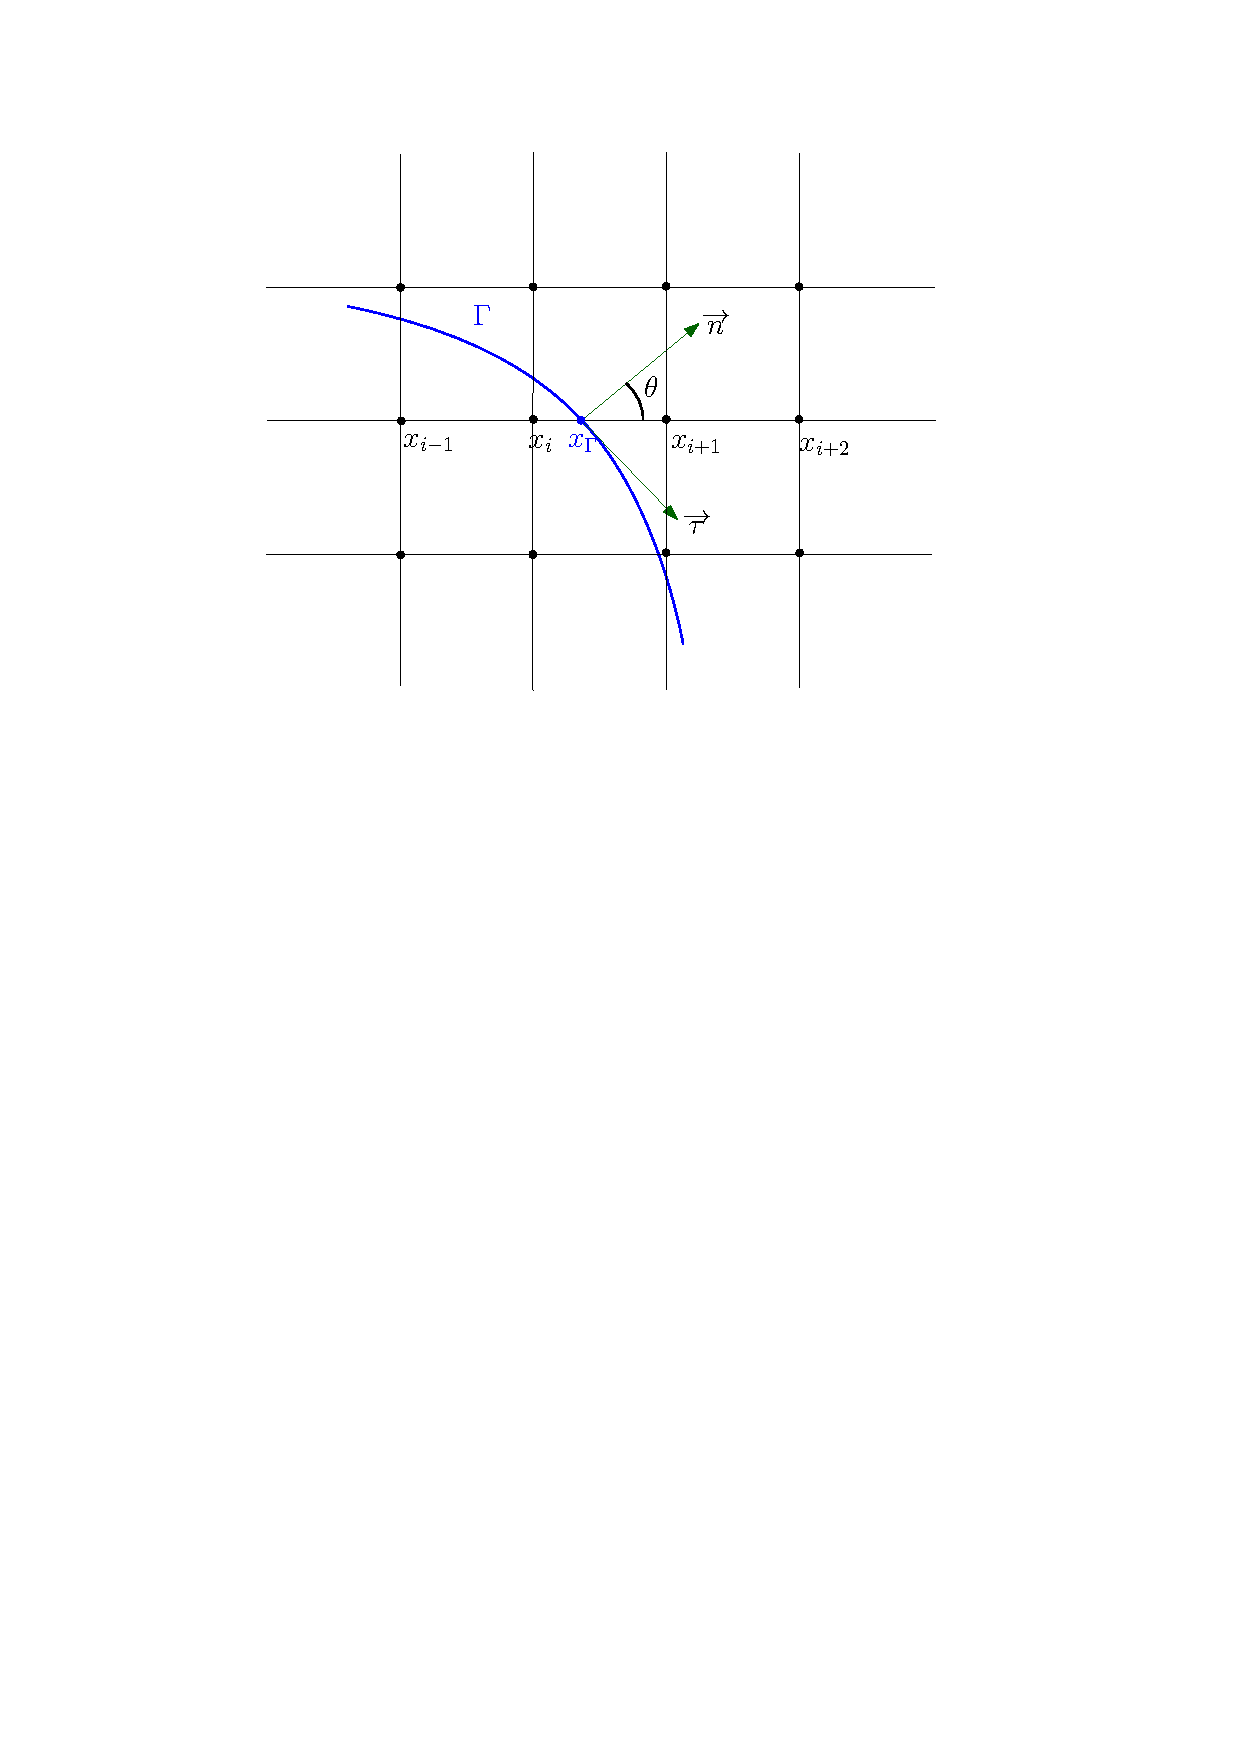
\includegraphics[width = 0.7\textwidth ]{GFM_2D.pdf}
\caption{2D GFM with the interface $\Gamma$ and the normal direction $\vec{n}$.}
\label{fig_gfm_2D}
\end{center}
\end{figure}

\begin{eqnarray}
\begin{aligned}
			\left[\epsilon \frac{\partial u}{\partial n}\right] &=& \cos \theta \left[\epsilon \frac{\partial u}{\partial x}\right] + \sin \theta \left[\epsilon \frac{\partial u}{\partial y}\right],\label{epun} \\
			\left[\epsilon \frac{\partial u}{\partial \tau}\right] &=& \sin \theta \left[\epsilon \frac{\partial u}{\partial x}\right] - \cos \theta\left[\epsilon \frac{\partial u}{\partial y}\right],\label{eput}	
\end{aligned}		
\end{eqnarray}
where $\theta$ is the angle between the normal direction and positive $x$ direction, as shown in Figure \ref{fig_gfm_2D}. 
Equation \ref{eput} can be solved for $ \left[\epsilon \frac{\partial u}{\partial x}\right]$ and $\left[\epsilon \frac{\partial u}{\partial y}\right]$:
\begin{eqnarray}
\begin{aligned}
	\left[\epsilon \frac{\partial u}{\partial x}\right] &=& \cos \theta \left[\epsilon \frac{\partial u}{\partial n}\right] +\sin \theta \left[\epsilon \frac{\partial u}{\partial \tau}\right],\label{epux1} \\
	\left[\epsilon \frac{\partial u}{\partial y}\right] &=& \sin \theta \left[\epsilon \frac{\partial u}{\partial n}\right] -\cos \theta \left[\epsilon \frac{\partial u}{\partial \tau}\right].\label{epuy1}
\end{aligned}	
\end{eqnarray}
To simplify the jump-conditions Liu, Fedkiw and Kang \cite{Liu2000}  smeared out the tangential derivative by considering $\left[\epsilon \frac{\partial u}{\partial \tau}\right]=0$ to get the following equations, 
%		\begin{eqnarray}
%			\left[\epsilon u_x\right] &=& \cos \theta \left[\epsilon u_n\right] \label{epux2}  \\
%			\left[\epsilon u_y\right] &=& sin \theta \left[\epsilon u_n\right] \label{epuy2}
%		\end{eqnarray}
\begin{eqnarray}
\begin{aligned}
	\left[\epsilon \frac{\partial u}{\partial x}\right] &\approx& \cos \theta \left[\epsilon \frac{\partial u}{\partial n}\right],\label{epux2}   \\
	\left[\epsilon \frac{\partial u}{\partial y}\right] &\approx& \sin \theta \left[\epsilon \frac{\partial u}{\partial n}\right], \label{epuy2}
\end{aligned}	
\end{eqnarray}
which are in general not true.
% but $\left[\epsilon \frac{\partial u}{\partial x}\right]$ and $\left[\epsilon \frac{\partial u}{\partial y}\right]$ in (\ref{epux2}) satisfies (\ref{epun}) for $\left[\epsilon \frac{\partial u}{\partial n}\right]$. 
It allows us to replace the unknown quantities as  $\left[\epsilon \frac{\partial u}{\partial x}\right]$ and $\left[\epsilon \frac{\partial u}{\partial y}\right]$ by the known quantities $\left[\epsilon \frac{\partial u}{\partial n}\right]$ and $\left[\epsilon \frac{\partial u}{\partial \tau}\right]$. This process used to simplify the jump condition in \cite{Liu2000} still requires the normal direction $\theta$. In our proposed GFM scheme  we have considered $\frac{\partial u^+}{\partial \tau}=0$ to get the following derivation for $ \left[\epsilon \frac{\partial u}{\partial x}\right] $:
\begin{eqnarray*}
\left[\epsilon \frac{\partial u}{\partial x}\right] &=& \cos \theta \left[\epsilon \frac{\partial u}{\partial n}\right] +\sin \theta \left[\epsilon \frac{\partial u}{\partial \tau}\right]\\
&=& \cos \theta \left[\epsilon \frac{\partial u}{\partial n}\right] +\sin \theta \left(\epsilon^+\frac{\partial u^+}{\partial \tau}-\epsilon^-\frac{\partial u^-}{\partial \tau}\right)\\
&=& \cos \theta\left[\epsilon \frac{\partial u}{\partial n}\right]+\sin \theta \left(\epsilon^+\frac{\partial u^+}{\partial \tau}-\epsilon^-\frac{\partial u^+}{\partial \tau}+\epsilon^-\frac{\partial u^+}{\partial \tau}-\epsilon^-\frac{\partial u^-}{\partial \tau}\right)\\
&=&\cos \theta\left[\epsilon \frac{\partial u}{\partial n}\right]+\sin \theta \left(\epsilon^-\left(\frac{\partial u^+}{\partial \tau}-\frac{\partial u^-}{\partial \tau}\right)+(\epsilon^+-\epsilon^-)\frac{\partial u^+}{\partial \tau}\right)\\
&=&\cos \theta\left[\epsilon \frac{\partial u}{\partial n}\right]+\sin \theta \left(\epsilon^-\left[\frac{\partial u}{\partial \tau}\right]+(\epsilon^+-\epsilon^-)\frac{\partial u^+}{\partial \tau}\right)
\end{eqnarray*}
Now by the jump conditions we have $ \left[\epsilon \frac{\partial u}{\partial n}\right] =\epsilon^- \frac{\partial G}{\partial n}$ and $\left[\frac{\partial u}{\partial \tau}\right]= \frac{\partial G}{\partial \tau}.$
\begin{eqnarray*}
\text{Thus } \left[\epsilon \frac{\partial u}{\partial x}\right] &=& \cos \theta (\epsilon^- \frac{\partial G}{\partial n})+\sin \theta .\epsilon^- \frac{\partial G}{\partial \tau} +\sin \theta (\epsilon^+ -\epsilon^- ) \frac{\partial u^+}{\partial \tau}\\
&\approx & \epsilon^-(\cos \theta  \frac{\partial G}{\partial n}+\sin \theta\frac{\partial G}{\partial \tau}) = \epsilon^- \frac{\partial G}{\partial x}\text{, if }\frac{\partial u^+}{\partial \tau}=0.\\
\text{Therefore, }\left[\epsilon \frac{\partial u}{\partial x}\right]&\approx &  \epsilon^- \frac{\partial G}{\partial x}.
\end{eqnarray*}
Similarly it can be shown that $\left[\epsilon \frac{\partial u}{\partial y}\right] \approx   \epsilon^- \frac{\partial G}{\partial y}$. Like the original GFM, our new GFM also omits some tangential information. Thus, two methods will have a local first order of truncation error. Nevertheless, in our new method, the normal direction of the complicated molecular surface is not required, so that the implementation of the modified GFM is much simpler than the standard GFM. 

%Now using  $\left[ u\right]= G$ from (\ref{phitilde3}) and $\left[\epsilon\frac{\partial u}{\partial x}\right]= \epsilon^-\frac{\partial G}{\partial x}$ from (\ref{phitilde4}) as the jump condition we have,
%%\begin{eqnarray}
%%	u^+-u^- &=& G\\
%%	\epsilon^+ u^+_x-\epsilon^- u^-_x &=& \epsilon^-\frac{\partial G}{\partial x}
%%\end{eqnarray}
%\begin{align*}
%	\tilde{u}_i&= \frac{\epsilon^-}{\epsilon^+\lambda+\epsilon^-(1-\lambda)}\textcolor{blue}{u_i} +\frac{\lambda(\epsilon^+-\epsilon^-)}{\epsilon^+\lambda+\epsilon^-(1-\lambda)}\textcolor{blue}{u_{i+1}}\\
%	&+\frac{\epsilon^-}{\epsilon^+\lambda+\epsilon^-(1-\lambda)} \textcolor{blue}{G}-\frac{h \lambda}{\epsilon^+\lambda+\epsilon^-(1-\lambda)}\textcolor{blue}{\epsilon^- \frac{\partial G}{\partial x}}\\
%	\tilde{u}_{i+1}&= \frac{(\epsilon^--\epsilon^+)(1-\lambda)}{\epsilon^+\lambda+\epsilon^-(1-\lambda)} \textcolor{blue}{u_i} +\frac{\epsilon^+}{\epsilon^+\lambda+\epsilon^-(1-\lambda)} \textcolor{blue}{u_{i+1}}\\
%	& -\frac{\epsilon^+}{\epsilon^+\lambda+\epsilon^-(1-\lambda)} \textcolor{blue}{G}-\frac{h(1-\lambda)}{\epsilon^+\lambda+\epsilon^-(1-\lambda)}\textcolor{blue}{ \epsilon^-\frac{\partial G}{\partial x}}
%\end{align*}


%%%%%%%%%%%%%%%%%%%%%%%%%%%%%%%%%%%%%%%%%%%%%%%%%%%%%%%%%%%%%%%%%%%%%%%%%%%%%

\section{Three dimensions}

Consider that the interface $\Gamma$ that intersects the grid line in the $x$ direction at a point $(i_\Gamma, j,k)$ which is located between $(i,j,k)$ and $(i+1,j,k)$, We therefore have two irregular grid points, $(i,j,k)$ and $(i+1,j,k)$. The fictitious values $\tilde{u}_{i,j,k}$ and $\tilde{u}_{i+1,j,k}$ are to be determined. To use one of the jump conditions which is defined in the normal direction of the interface point, it is convenient to introduce a local coordinates $(\xi,\eta,\zeta)$ such that $\xi$ is along the normal direction and $\eta $ is in the $xy$ plane. Then the coordinate transformation can be given as, 
\begin{align}
  \left[
            \begin{array}{c}
             x\\
             y\\
             z
       \end{array}\right] =\bf{P}\left[\begin{array}{c}
            \xi\\
            \eta\\
            \zeta
     \end{array}\right],\label{eqtran1}
\end{align}
%\begin{align}
%    \left[\begin{array}{c}
%            \xi\\
%            \eta\\
%            \zeta
%     \end{array}\right]=\bf{P}\left[
%            \begin{array}{c}
%             x\\
%             y\\
%             z
%       \end{array}\right],\label{eqtran1}
%\end{align}
where $\bf{P}$ is the transformation matrix
%\begin{align}
%    \bf{P}=\left[\begin{array}{ccc}
%                 \sin\psi\cos\theta & \sin\psi\sin\theta & \cos\psi\\
%                 -\sin\theta        & \cos\theta         & 0       \\
%                 -\cos\psi\cos\theta&-\cos\psi\sin\theta & \sin\psi
%                 \end{array}\right]. \label{eqtran2}
%\end{align}
\begin{align}
    \bf{P}=\left[\begin{array}{ccc}
                 \sin\psi\cos\theta  &-\sin\theta   & -\cos\psi\cos\theta \\
                \sin\psi\sin\theta   & \cos\theta   & -\cos\psi\sin\theta \\
                  \cos\psi 			 & 0 			& \sin\psi
                 \end{array}\right]. \label{eqtran2}
\end{align}
Here $\theta$ and $\psi $ are the azimuth and zenith angles with respect to the normal direction $\xi$.
% Now to express the jump condition along x-axis $\left[\epsilon \frac{\partial u}{\partial x}\right]$  in terms of $\left[\epsilon \frac{\partial u}{\partial \xi}\right]$, $\left[\epsilon \frac{\partial u}{\partial \eta}\right]$ and $\left[\epsilon \frac{\partial u}{\partial \zeta}\right]$ we have 
Then from equation (\ref{eqtran1}) and (\ref{eqtran2}) we have, 
\begin{eqnarray}
	\left[\epsilon \frac{\partial u}{\partial x}\right] &=& \sin \psi \cos \theta \left[\epsilon \frac{\partial u}{\partial \xi}\right]-\sin \theta \left[\epsilon \frac{\partial u}{\partial \eta}\right]-\cos \psi \cos \theta \left[\epsilon \frac{\partial u}{\partial \zeta}\right]\label{3d_gfm1}
\end{eqnarray}
Now along the $\eta$ axis,
\begin{eqnarray}
\begin{aligned}
	\left[\epsilon \frac{\partial u}{\partial \eta}\right] &= \epsilon^+\frac{\partial u^+}{\partial \eta }-\epsilon^-\frac{\partial u^-}{\partial \eta }\\
	&=\epsilon^+\frac{\partial u^+}{\partial \eta }-\epsilon^-\frac{\partial u^+}{\partial \eta }+\epsilon^-\frac{\partial u^+}{\partial \eta }-\epsilon^-\frac{\partial u^-}{\partial \eta }\\
	&= \epsilon^-\left(\frac{\partial u^+}{\partial \eta }-\frac{\partial u^-}{\partial \eta }\right)+(\epsilon^+-\epsilon^-)\frac{\partial u^+}{\partial \eta}\\
	&= \epsilon^-\frac{\partial G}{\partial \eta}+(\epsilon^+-\epsilon^-)\frac{\partial u^+}{\partial \eta}\text{ since } \left(\frac{\partial u^+}{\partial \eta }-\frac{\partial u^-}{\partial \eta }\right)=\frac{\partial}{\partial\eta}[u]=\frac{\partial G}{\partial \eta}.\label{3d_gfm2}
\end{aligned}
\end{eqnarray}
Similarly along the $\zeta $ axis, 
\begin{equation}
	\left[\epsilon \frac{\partial u}{\partial \zeta}\right]= \epsilon^-\frac{\partial G}{\partial \zeta}+(\epsilon^+-\epsilon^-)\frac{\partial u^+}{\partial \zeta }.\label{3d_gfm3}
\end{equation}
Then from equations (\ref{3d_gfm1}), (\ref{3d_gfm2}) and (\ref{3d_gfm3}) we have,
\begin{eqnarray}
\begin{aligned}   
		\left[\epsilon \frac{\partial u}{\partial x}\right]&= \epsilon^-\left( \sin \psi \cos \theta \frac{\partial G}{\partial \xi}-\sin \theta \frac{\partial G}{\partial \eta}-\cos \psi \cos \theta \frac{\partial G}{\partial \zeta}\right)\\
		 &-\sin\theta (\epsilon^+-\epsilon^-)\frac{\partial u}{\partial \eta}^+ -\cos{\phi} \cos \theta (\epsilon^+-\epsilon^-) \frac{\partial u^+}{\partial \zeta }\\
		 &=\epsilon^- \frac{\partial G}{\partial x}-\sin\theta (\epsilon^+-\epsilon^-)\frac{\partial u}{\partial \eta}^+ -\cos{\phi} \cos \theta (\epsilon^+-\epsilon^-) \frac{\partial u^+}{\partial \zeta }\\
		 &\approx \epsilon^- \frac{\partial G}{\partial x}\text{     assuming } \frac{\partial u}{\partial \eta}^+ =0 \text{ and } \frac{\partial u^+}{\partial \zeta }=0.  
\end{aligned}\label{eq:m-gfm1}		  	
\end{eqnarray}
Similarly along $y$ axis and $z$ axis from equation (\ref{3d_gfm1}),(\ref{3d_gfm2}) and (\ref{3d_gfm3}) we have:
\begin{eqnarray}
\begin{aligned}  
\left[\epsilon \frac{\partial u}{\partial y}\right]\approx\epsilon^- \frac{\partial G}{\partial y}\text{ and } \left[\epsilon \frac{\partial u}{\partial z}\right]\approx\epsilon^- \frac{\partial G}{\partial z}.\label{eq:m-gfm2}
\end{aligned}		  	
\end{eqnarray}
%%%%%%%%%%%%%%%%%%%%%%%%%%%%%%%%%%%%%%%%%%%%%%%%%%%%%%%%%%%%%%%%%%%%%%%%%%%%%

\section{Corner point for the modified GFM method}
% TODO Maybe have to describe more about Corner point
We have a special situation for a corner point when the interface crosses the grid line for the same axis twice around $x_i$ where $x_{i-1}$ and $x_{i+1}$ are on the other side of the interface as shown in Figure \ref{fig:corner_point}. There are two types of corner point situations. In one type the point $x_i$ is in $\Omega^-$ and the other two adjacent points are in $\Omega^+$ (see Figure \ref{fig:corner_point}). For this case we define $G_L=-G$ and $G_R = G$ to derive the following equations for the fictitious points $\tilde{u}_{i-1}$ and $\tilde{u}_{i+1}$: 
\begin{figure}[!h]		
\begin{center}
	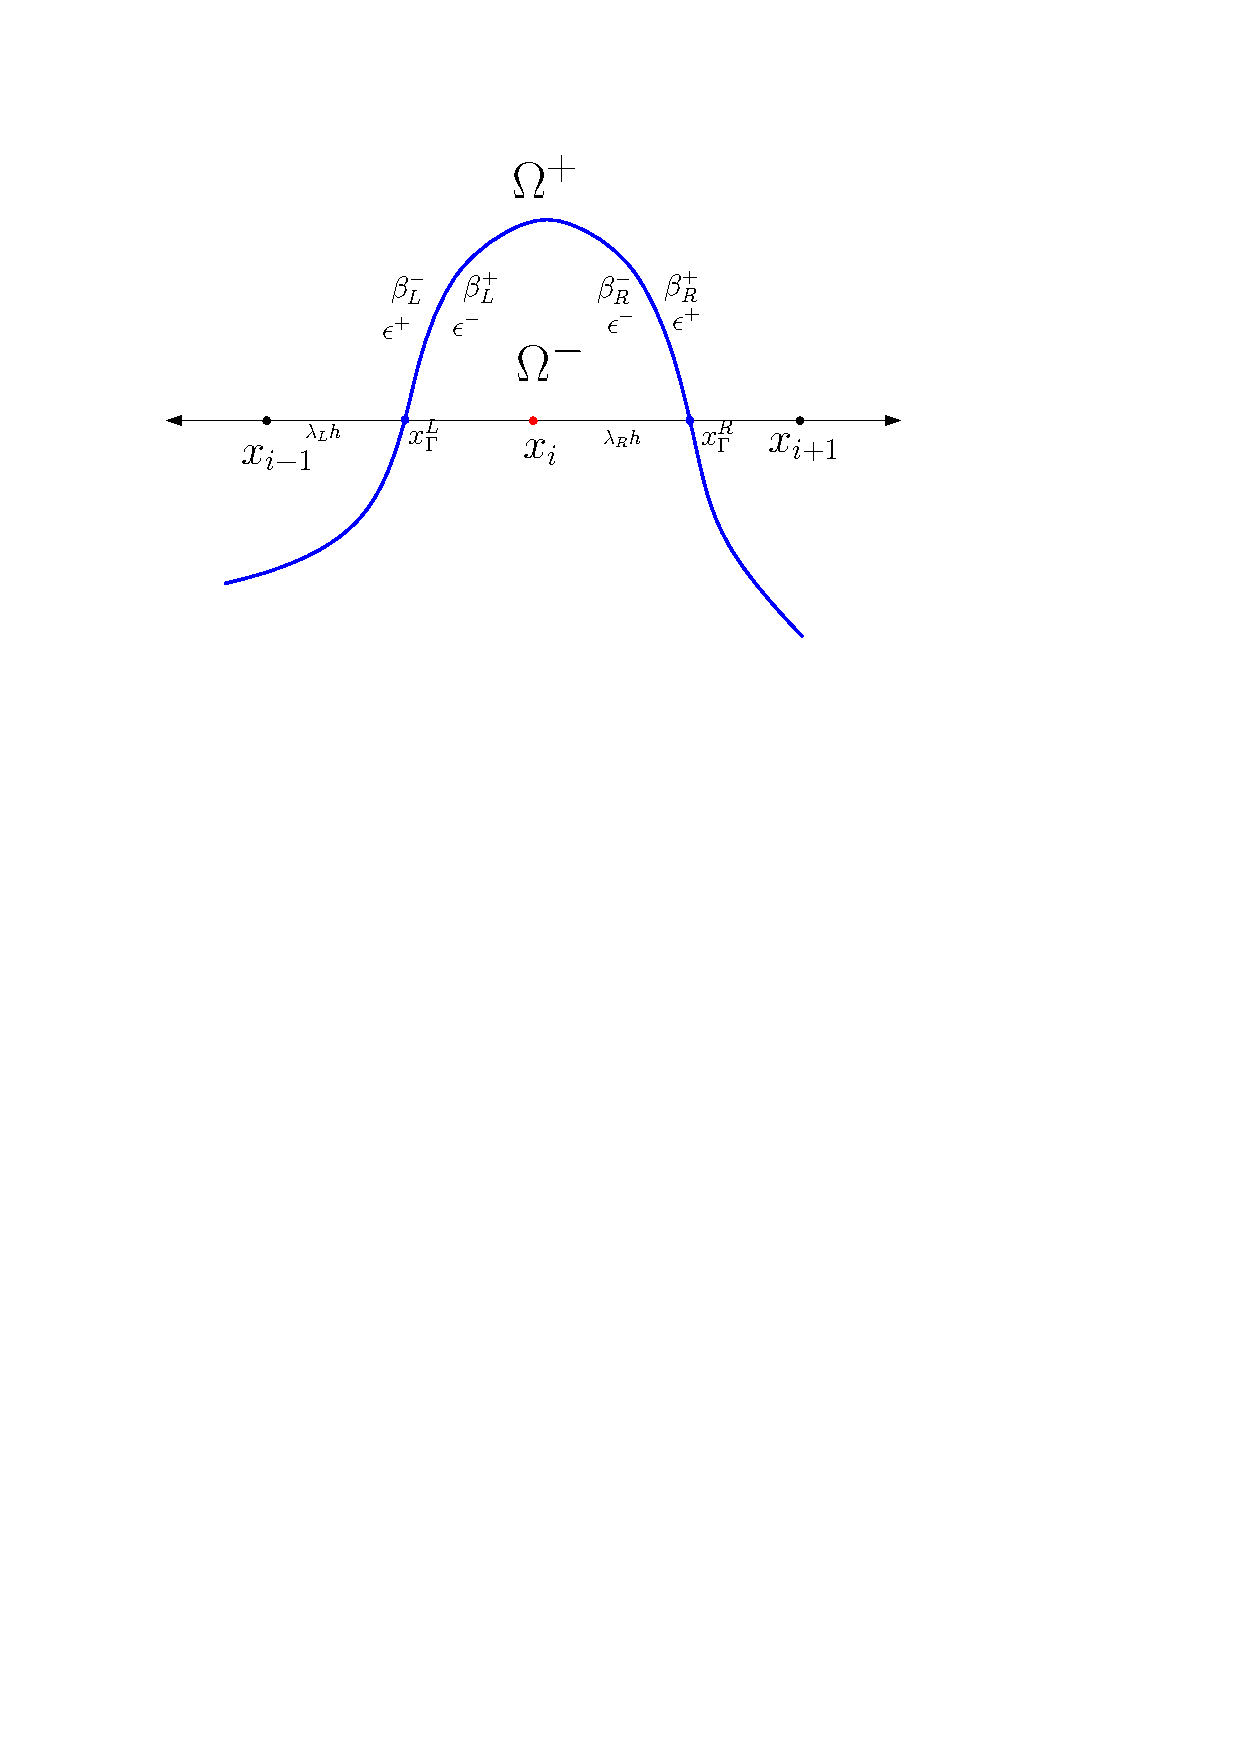
\includegraphics[width = 0.7\textwidth ]{GFMcorner.pdf}		
\end{center}
\caption{2D representation for a corner point treatment for the point $x_i$ }
\label{fig:corner_point}
\end{figure}
\begin{equation}
	\tilde{u}_{i-1}= A_1 u_{i-1}+B_1 u_{i} + C_1 G_L- D_1 \epsilon^- \frac{\partial G_L}{\partial x},\label{eq:corner1}
\end{equation}
and
\begin{equation}	
	\tilde{u}_{i+1}= A_2 u_{i+1}+B_2 u_{i} - C_2 G_R- D_2 \epsilon^- \frac{\partial G_R}{\partial x},\label{eq:corner2}
\end{equation}
where,
    $$	A_1 = \frac{\beta^-_L}{F_1}, B_1  = \frac{\lambda_L(\beta^+_L-\beta^-_L)}{F_1}, C_1 = \frac{\beta^-_L}{F_1},D_1 = \frac{h \lambda_L}{F_1}, $$ %, 
	$$A_2 = \frac{\beta^+_R}{F_2}, B_2  = \frac{(1-\lambda_R)(\beta^-_R-\beta^+_R)}{F_2}, C_2 = \frac{\beta^+_R}{F_2},D_2 = \frac{h(1- \lambda_R)}{F_2},$$
	$$\beta_L^-=\epsilon^+,\beta_L^+=\epsilon^-,\beta_R^-=\epsilon^-,\beta_R^+=\epsilon^+,$$
	$$\lambda_L=\frac{x^L_\Gamma-x_{i-1}}{h},\lambda_R=\frac{x^R_\Gamma-x_i}{h},$$
	$$F_1 = \beta^+_L \lambda_L+\beta^-_L(1-\lambda_L), F_2 = \beta^+_R \lambda_R+\beta^-_R(1-\lambda_R).$$
For the other type of the corner points we have the point $x_i$ in $ \Omega^+$ with its adjacent points in $x$ direction in $\Omega^-$. We can use the similar type of calculation like the previous type of corner points considering $G_L=G$ and $G_R = -G$ to find the factious points using the equations (\ref{eq:corner1}) and (\ref{eq:corner2}). 

	
%%%%%%%%%%%%%%%%%%%%%%%%%%%%%%%%%%%%%%%%%%%%%%%%%%%%%%%%%%%%

\section{Simplicity of the modified GFM}

Altogether this proposed modified GFM is much more easier to program compared to the MIB method used in \cite{Zhihan2017}. Unlike the MIB method, the modified GFM doesn't need to generate local coordinates in the non-orthogonal tangential directions. We are also avoiding the tensor product decomposition of jump conditions used in mADI\cite{Zhihan2017} by the approximate jump conditions proposed in equations (\ref{eq:m-gfm1}) and (\ref{eq:m-gfm2}). At the end we are only using the three points on the finite difference stencil and its not necessary to consider any other auxiliary points to calculate any approximation of tangential derivatives like mADI does.    

We have also simplified the step to get the axial direction jump conditions from the normal direction jump conditions. For the original GFM method in \cite{Liu2000}, Liu, Fedkiw and Kang needed the angle $\theta$ between the normal direction and the axial directions for this process which is not required for the modified GFM method. This reduces the required amount of information about the molecular surface. 